\graphicspath{{images/pangenomeAnalysis/}{images/phylogeneticStructureHostData}}


\begin{figure}[h!] 
     \centering
     \begin{subfigure}[b]{0.45\textwidth}
        \centering
        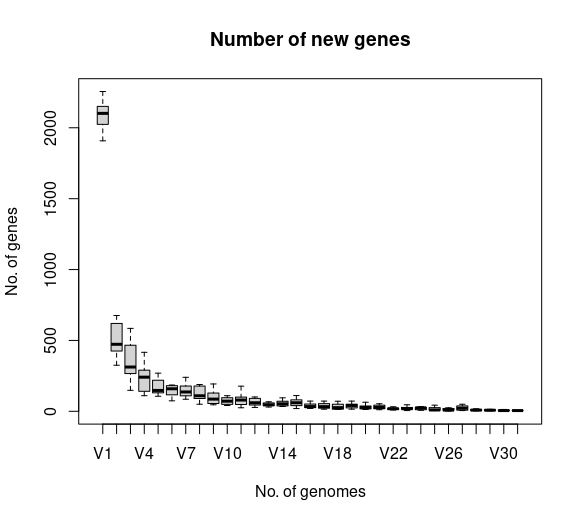
\includegraphics[width=\textwidth]{number_new_genes}
        \caption{Number of new genes}
        \label{fig:new genes}
     \end{subfigure}
     \hfill
     \begin{subfigure}[b]{0.45\textwidth}
        \centering
        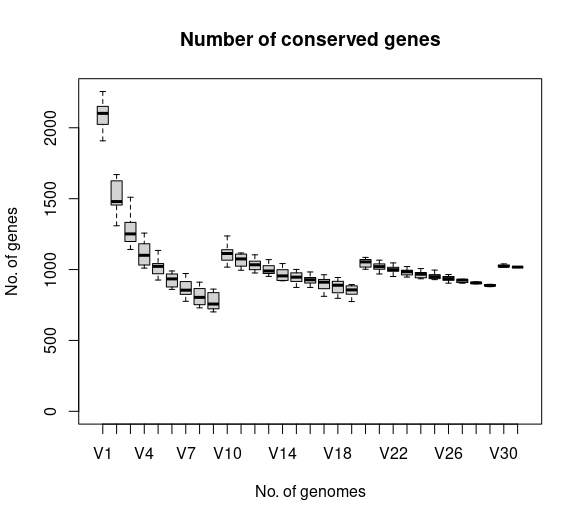
\includegraphics[width=\textwidth]{number_conserved_genes}
        \caption{Number of conserved genes}
        \label{fig:conserved genes}
     \end{subfigure}
     \hfill
     \begin{subfigure}[b]{0.45\textwidth}
        \centering
        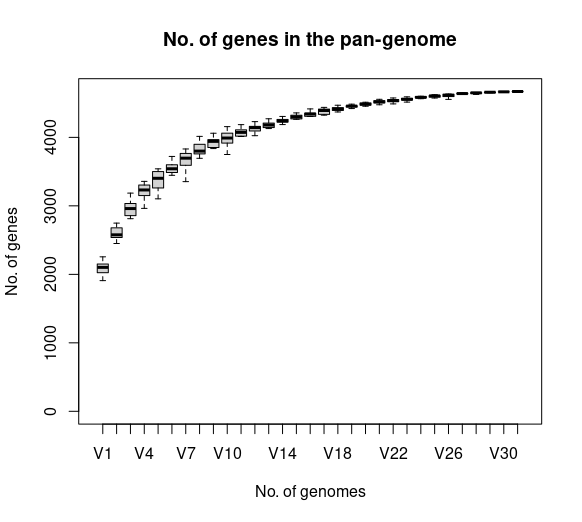
\includegraphics[width=\textwidth]{number_genes_pangenome}
        \caption{Number of genes in the pan-genome}
        \label{fig:pagenome genes}
     \end{subfigure}
     \hfill
     \begin{subfigure}[b]{0.45\textwidth}
        \centering
        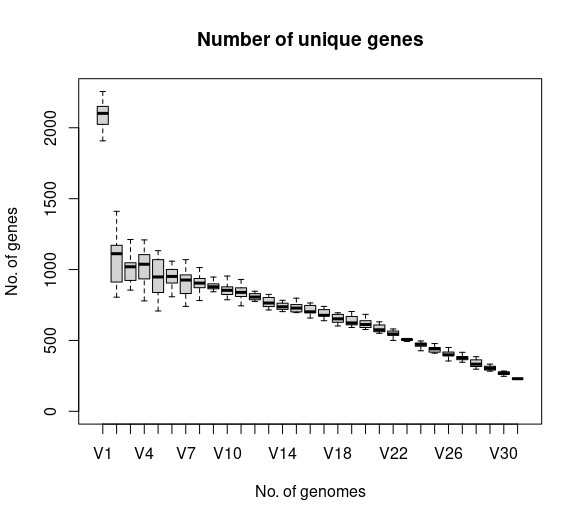
\includegraphics[width=\textwidth]{number_unique_genes}
        \caption{Number of unique genes}
        \label{fig:unique genes}
     \end{subfigure}
     \hfill
      \caption{\footnotesize{Plots obtained from the output of the pangenome anotation with Roary. The number of new \textbf{(a)}, conserved
      \textbf{b}}, total \textbf{c} and unique \textbf{d} genes show consistent and 
      expected trend as the number of considered genomes increases.}
      \label{fig:genes vs genomes}
\end{figure}




\begin{figure}
   \centering
   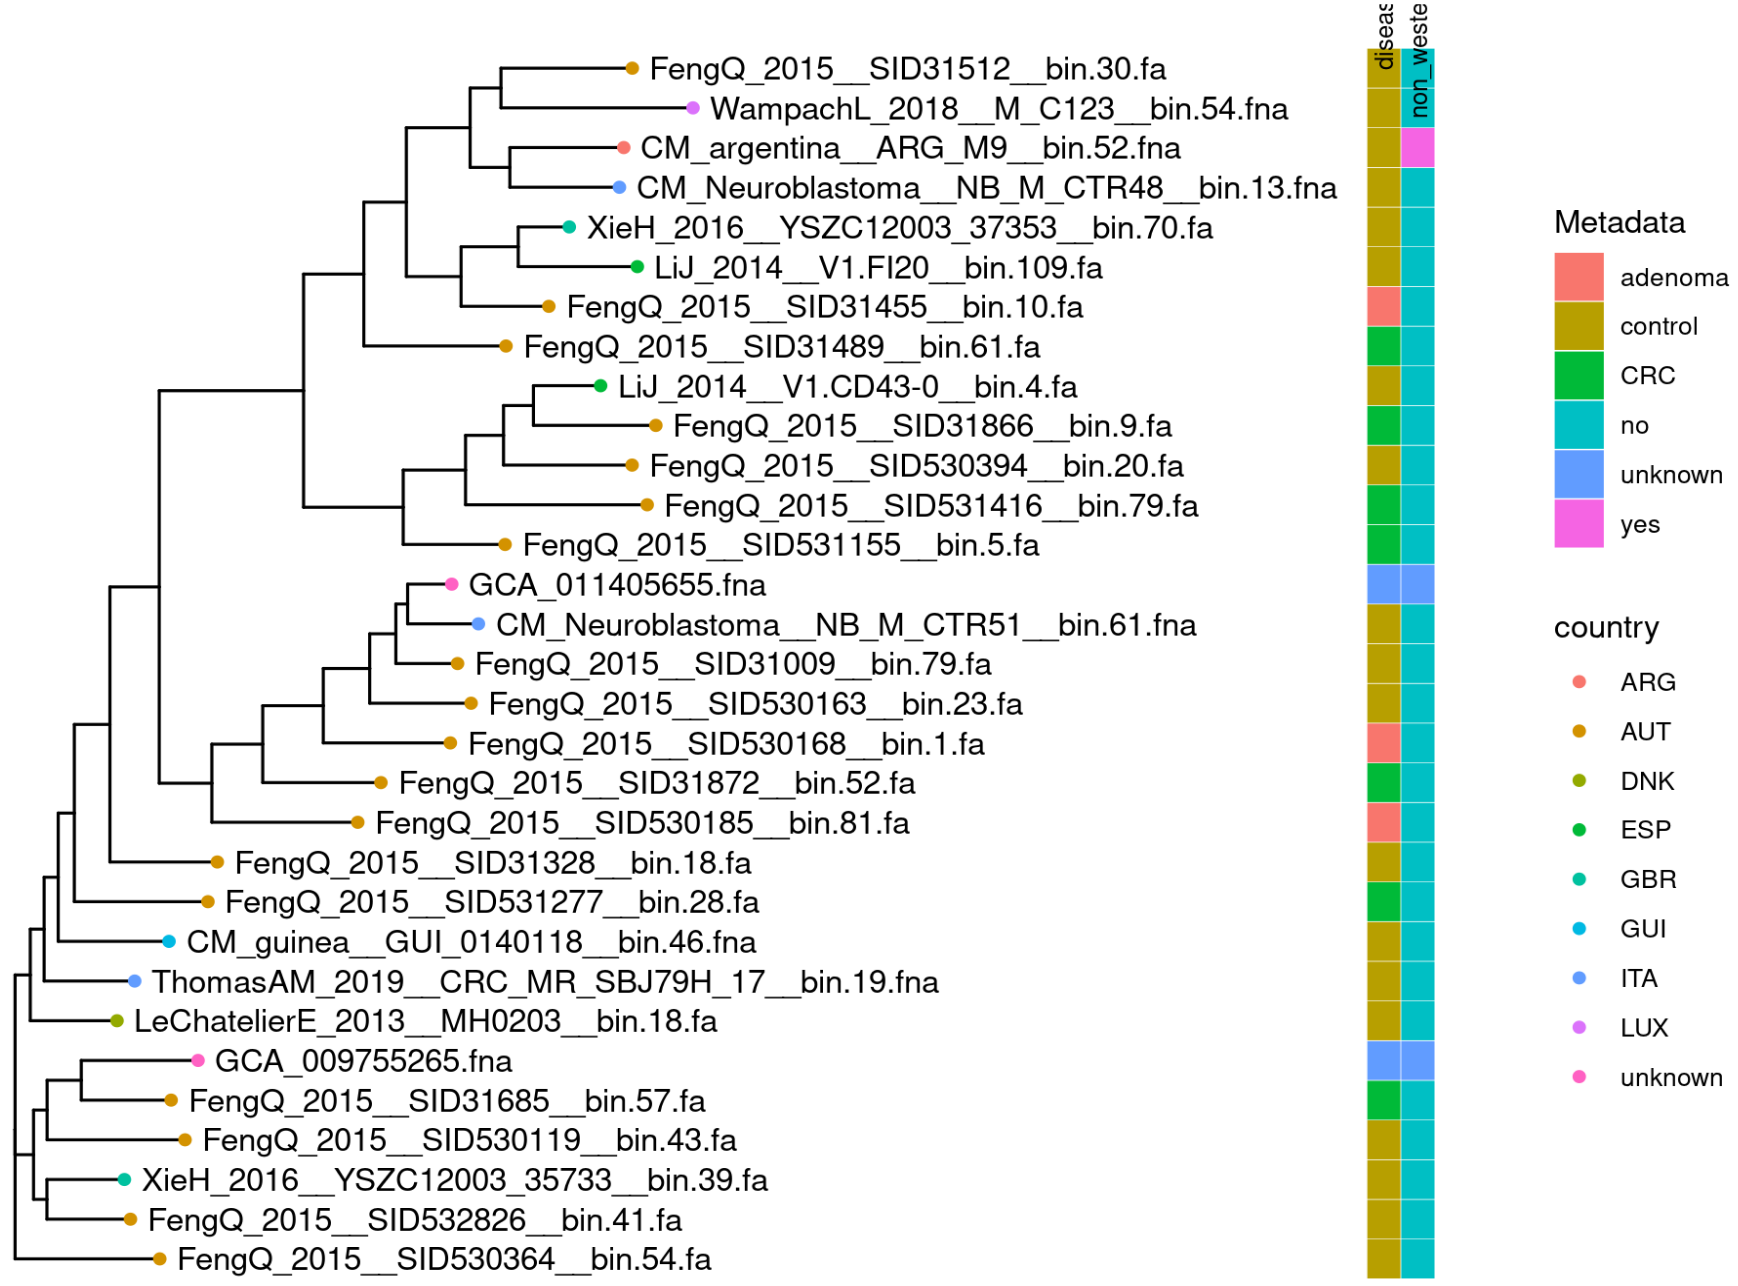
\includegraphics[width=0.8\textwidth]{enriched_tree_fromMafft_final.png}
   \caption{\footnotesize{Tree generated from the core gene alignement
   obtained using MAFFT with the colour of the tip representing the country
   of provenence of the host; the heatmap shows the disease and the classification as 
   non-westernized (NW) of the host.}}
   \label{core alignement mafft tree}
\end{figure}


